\documentclass[12 pt]{article}
%%%%%%%%%%%%%%%%%%%%%%%%%%%%
%\topmargin 0.2in
%\textheight 10in
%\voffset -1.25in
%\textwidth 6.2in
%\parindent 0.25in
%\itemindent 0.in
%\leftmargin 0.5in
%\hoffset -0.8in

%\addtolength{\textwidth}{ain}
%\addtolength{\hoffset}{-bin}
%\addtolength{\textheight}{cin}
%\addtolength{\voffset}{cin}
%a=2b

\addtolength{\textwidth}{1.in}
\addtolength{\hoffset}{-.5in}
\addtolength{\textheight}{1.in}
\addtolength{\voffset}{-1.in}


%Packages
\usepackage{graphicx}
\usepackage[mathcal,mathscr]{eucal}
\usepackage{amsfonts}
\usepackage{mathrsfs}
\usepackage{amsmath, amsthm, amssymb,epsfig,amscd,multicol}
\usepackage{enumitem}
\usepackage{xcolor}
\usepackage{tikz}
\usetikzlibrary{arrows,positioning,shapes,fit}
\usepackage{float}
\usepackage{caption}
\usepackage{subcaption}
\usepackage[style=1]{mdframed}
%\usepackage{tabu}
\usepackage{arydshln}
\usepackage{cancel}
%\usepackage{mathptmx}

%New Commands
\newcommand{\R}{\mathbb{R}}
\newcommand{\Z}{\mathbb{Z}}
\newcommand{\Q}{\mathbb{Q}}
\newcommand{\N}{\mathbb{N}}
\renewcommand{\P}{\mathscr{P}}
\newcommand{\set}[1]{\left\{#1\right\}}
\newcommand{\ds}{\displaystyle}
\newcommand{\diff}[2]{\frac{d #1}{d #2}}
\renewcommand{\subset}{\subseteq} 
\newcommand{\divides}{\! \mid \!}
\newcommand{\ndivides}{\! \nmid \!}
\newcommand{\mymod}[1]{ \ (\bmod \ #1)}
\newcommand{\esub}{\subseteq}
\newcommand{\rel}{\mathbin{R}}

\theoremstyle{definition}
\newtheorem{remark}{Remark}

\theoremstyle{plain}

\newtheoremstyle{mytheorem}% name of the style to be used
  {6pt}% measure of space to leave above the theorem. E.g.: 3pt
  {6pt}% measure of space to leave below the theorem. E.g.: 3pt
  {\itshape}% name of font to use in the body of the theorem
  {0pt}% measure of space to indent
  {\bfseries}% name of head font
  {.}% punctuation between head and body
  {5 pt plus 1pt minus 1pt}% space after theorem head; " " = normal interword space
  {}% Manually specify head
  
 	\theoremstyle{mytheorem}
  	\newtheorem{theorem}{Theorem}[section]%[numbering]
	\newtheorem{lemma}{Lemma}
	\newtheorem{cor}{Corollary}[section]
	
	

\newtheoremstyle{myexample}% name of the style to be used
  {22pt}% measure of space to leave above the theorem. E.g.: 3pt
  {22pt}% measure of space to leave below the theorem. E.g.: 3pt
  {\normalfont}% name of font to use in the body of the theorem
  {0pt}% measure of space to indent
  {\bfseries}% name of head font
  {.}% punctuation between head and body
  {5 pt plus 1pt minus 1pt}% space after theorem head; " " = normal interword space
  {}% Manually specify head

	\theoremstyle{myexample}
	\newtheorem{example}{Example}[section]
	\newtheorem{claim}{Claim}
	
	
\newtheoremstyle{mydefinition}% name of the style to be used
  {12pt}% measure of space to leave above the theorem. E.g.: 3pt
  {12pt}% measure of space to leave below the theorem. E.g.: 3pt
  {\normalfont}% name of font to use in the body of the theorem
  {0pt}% measure of space to indent
  {\bfseries}% name of head font
  {.}% punctuation between head and body
  {5 pt plus 1pt minus 1pt}% space after theorem head; " " = normal interword space
  {}% Manually specify head

	\theoremstyle{mydefinition}
	\newtheorem{definition}{Definition}
	\newtheorem*{definition*}{Definition}





\begin{document}
\pagenumbering{gobble}
\begin{center}
\textbf{Which is bigger: $\R$ or $\R^2$?\\
They're the same?  Nevermind then.  }
\end{center}



\section{Comparing Infinite Cardinalities}

We have worked out that $|\N| \neq |(0,1)|$.  This means we definitely have two different types of infinity, but how do they compare?  Recall that we showed $|\N| \neq |(0,1)|$ by showing that it's impossible to list the unit interval in an ordered way.  What this means is that we cannot provide a surjective function from $\N$ to $(0,1)$.  

	\begin{enumerate}[resume]
	\item Provide a surjective function $f:(0,1) \to \N$.  Is your function injective?  Do you think it's possible to find an injective function?
	
	\vspace{1.5in}
	\end{enumerate}
	
With this last example in mind, we define what it means to compare sets with infinite cardinalities.

\begin{definition}  Suppose $A$ and $B$ are infinite sets.  We say $|A|<|B|$ if there are injective functions from $A$ to $B$, but no surjective functions from $A$ to $B$.  We say $|A|>|B|$ if there are surjective functions from $A$ to $B$, but no injective functions.
\end{definition}

In general, proving that there are no surjections between infinite sets is quite difficult.  For instance,  it seems like it should be easy to prove that $|\R^2|>|\R|$, but in reality $|\R|=|\R^n|$ for all $n \in \N$ (look up Hilbert's Curve for details).  When we start dealing with infinities, we just can't trust our intuition anymore.  Let's explore one of the simpler examples.

\begin{claim}  If $A$ is any set, then $|A|< |\P(A)|$.
\end{claim}

\noindent Let's work out a proof for Claim 1.
\begin{mdframed}[backgroundcolor=gray!10!]
\begin{proof}
Let $A$ be a set.\\
\begin{mdframed}[backgroundcolor=white]
\begin{enumerate}[resume]
\item The claim doesn't require that $A$ be finite or infinite, so we should consider both cases.  Prove that if $A$ is finite, then $|A|<|\P(A)|$.
\vspace{2in}

\item When $A$ is infinite, things get a little more complicated because $\P(A)$ is infinite as well.  Recall that our goal is to show that there are injective functions from $A$ to $\P(A)$, but no surjective functions from $A$ to $\P(A)$.  Provide an injective function from $A$ to $\P(A)$.  If you construct a sensible function, it should be clear it's injective without a proof.
\vspace{2in}

\item We now need to show that there are no surjections from $A$ to $\P(A)$.
\end{enumerate}
\end{mdframed}
For sake of contradiction, suppose $f: A \to \P(A)$ is a surjection.  Notice, if $x \in A$ then $f(x) \in \P(A)$.\\
\begin{mdframed}[backgroundcolor=white]
\begin{enumerate} \setcounter{enumi}{4}
\item Why is the above statement true?
\vspace{.5in}
\item If $f(x) \in \P(A)$, then what else must be true about $f(x)$?  (Think about what a power set is.)
\vspace{.5in}
\end{enumerate}
\end{mdframed}
\noindent Since $f$ sends elements of $A$ to subsets of $A$, for $x \in A$ we can say either $x \in f(x)$ or $x\notin f(x)$.  With this in mind, we construct the set
\[B = \set{x \in A : x \notin f(x)} \esub A.\]
Since $B \esub A$, it must be true that $B \in \P(A)$.  Since $f$ is assumed to be a surjection, there exists $a \in A$ such that $f(a) = B$.\\
\begin{mdframed}[backgroundcolor=white]
\begin{enumerate}\setcounter{enumi}{6}
\item Suppose $a \in B$.  What can you say about $a$?

\vspace{3in}
\item Suppose $a \notin B$.  What can be said about $a$?

\vspace{3in}
\end{enumerate}
\end{mdframed}
\end{proof}
\end{mdframed}
\section{The Pigeonhole Principle}
Finally, we explore a relatively simple concept that can be used to write some interesting proofs.  Colloquially, the Pigeonhole Principle says that if you have fewer pigeons than you do pigeonholes and each pigeon goes to at least one hole, then at least one hole contains more than one pigeon.  Or, if you have more holes than pigeons, at least one hole contains no pigeons.  The principle is stated more formally below.\\

\noindent \textbf{The Pigeonhole Principle:}  Suppose $A$ and $B$ are sets and $f: A \to B$ is any function.
	\begin{enumerate}[label=(\arabic*)]
	\item If $|A|>|B|$ then $f$ is not injective.
	\item If $|A|<|B|$ then $f$ is not surjective.
	\end{enumerate}


\begin{center}
\begin{multicols}{2}
\resizebox{!}{2.5in}{	
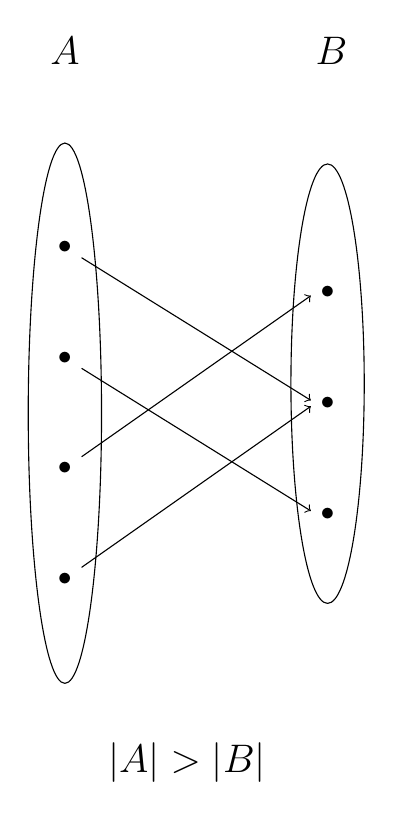
\begin{tikzpicture}
\node (a1){$\bullet$};
\node[above=2cm of a1] (title1){\Large $A$};
\node[below=of a1] (a2){$\bullet$};
\node[below=of a2] (a3){$\bullet$};
\node[below=of a3] (a4){$\bullet$};
\node[shape=ellipse,draw=black,fit={(a1) (a4)}]{};

\node [right=3cm of a1](space){};
\node [right=2.75cm of title1](title2){\Large $B$};
\node [below=.25cm of space](b1){$\bullet$};
\node [below=of b1](b2){$\bullet$};
\node [below=of b2](b3){$\bullet$};
\node[shape=ellipse,draw=black,fit={(space) (b3)}]{};

\draw[->,black] (a1)--(b2.170);
\draw[->,black] (a2)--(b3.170);
\draw[->,black] (a3)--(b1.190);
\draw[->,black] (a4)--(b2.190);

\node[below=2cm of a4](space2){};
\node[right=.3cm of space2]{\Large $|A|>|B|$};
\end{tikzpicture}}


\resizebox{!}{2.5in}{	
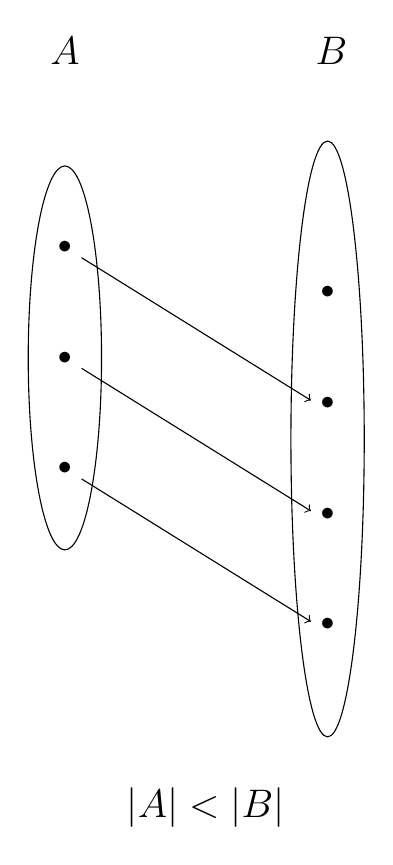
\begin{tikzpicture}
\node (a1){$\bullet$};
\node[above=2cm of a1] (title1){\Large $A$};
\node[below=of a1] (a2){$\bullet$};
\node[below=of a2] (a3){$\bullet$};
\node[shape=ellipse,draw=black,fit={(a1) (a3)}]{};

\node [right=3cm of a1](space){};
\node [right=2.75cm of title1](title2){\Large $B$};
\node [below=.25cm of space](b1){$\bullet$};
\node [below=of b1](b2){$\bullet$};
\node [below=of b2](b3){$\bullet$};
\node [below=of b3](b4){$\bullet$};
\node[shape=ellipse,draw=black,fit={(space) (b4)}]{};

\draw[->,black] (a1)--(b2.170);
\draw[->,black] (a2)--(b3.170);
\draw[->,black] (a3)--(b4.170);

\node[below=2cm of b4](space2){};
\node[left=.3cm of space2]{\Large $|A|<|B|$};
\end{tikzpicture}}
\end{multicols}
\end{center}

This property shouldn't seem particularly surprising.  Humans have a relatively strong inherent sense of numbers, and even children just learning to count have some rudimentary understanding of this concept.  Let's define a new type of set to play with the Pigeonhole Principle.

\begin{definition}[$\Z_p$]  Suppose $p$ is a prime number.  We define $\Z_p$ to be the set $\set{0,1,\ldots,p}$.
\end{definition}

Notice that $\Z_p$ contains all of the possible remainders when dividing by $p$.

\begin{enumerate}\setcounter{enumi}{8}
\item Let $p$ be any prime and prove that any function from $\Z_p$ to $\N$ is not surjective.
\end{enumerate}

\vspace{2in}

\noindent Below is an interesting use of the Pigeonhole Principle.

\begin{claim}  If $A$ is any set of 9 numbers with values between 1 and 50 (with repeats allowed), then there are two subsets of $A$, $X$ and $Y$ with $X\neq Y$ for which the sum of the elements of $X$ is the same as the sum of the elements of $Y$. 
\end{claim}

As an example, let $A=\set{1,3,7,11,12,17,23,31,42}$.  We could have $X = \set{11,12}$ and $Y=\set{23}$ or $X=\set{12,23}$ and $Y=\set{1,3,31}$.

\begin{mdframed}[backgroundcolor=gray!10!]
\begin{proof} Let $A$ be a set of 9 numbers with values between 1 and 50.

\begin{mdframed}[backgroundcolor=white]
\begin{enumerate} \setcounter{enumi}{9}
\item What is the largest possible value for the sum of the elements of $A$?  What about the smallest?  Remember that repeats are allowed.
\vspace{.5in}
\item How large is the power set of $A$?  (You'll actually need to know the value.)
\vspace{.5in}
\end{enumerate}
\end{mdframed}
Define the function $f: \P(A) \to \set{9,10,\ldots,450}$ as the sum of the elements in the set.  (So $f(\set{1,2,3})=6.$  Notice that $f$'s inputs are sets and not individual numbers).\\
\begin{mdframed}[backgroundcolor=white]
\begin{enumerate} \setcounter{enumi}{11}
\item What does the Pigeonhole Principle tell you about $f$?  What can you conclude?
\vspace{3in}
\end{enumerate}
\end{mdframed}
\end{proof}
\end{mdframed}
\end{document}




